\section{STEADY-STATE THERMAL ANALYSIS}
\normalsize{Steady-state thermal analysis is the main type of analysis that was carried out to analyse the different components of the \acrshort{ECRH} \acrshort{TZM}-reflector tile assembly. Different scenarios and loadcases were designed to give insight on the thermal behavior and performances of the tile, that being, the impact of the design changes of the \acrshort{TZM}-reflector tile, the influences of different \acrshort{ECRH} beam configurations or the influences of the film coefficient in the cooling pipe.}
\subsection{Calculation of the surface integrales} \label{Calculation of the surface integrales}
\normalsize{To compare between the old and new tile design but also validate the finite element model, calculating the surface integral can be of use. This idea behind this is to check for energy conservation after integration the heat flux of the \acrshort{ECRH} beam on the tile surface. Analytical calculations are a good approach to estimate the overall heat flow through the \acrshort{TZM} tile. After the calculation of the surface integrales ($\it{see}$ \ref{MODELLING OF THE ECRH BEAM}), it is possible to numerically estimate an integral and predictict the heat flux through the old and the new design.}
\\
\break
\normalsize{\indent The surface onto which the heat disribution is integrated is a rough approximation of the surface of the \acrshort{TZM} tile (the projected area of the tile was simplified to a rectangle of size $95mm \times 95mm$). The function is then integrated using a Wolfram Mathematica\textsuperscript{\textregistered} script. To evaluate the validity of the analytical calculation, a finite element model including only the old and the new \acrshort{TZM} tile was developed to calculate the surface integral but using the finite element method. The idea is to compare both methods to estimate the heat flow. }
\\
\begin{figure}[h!]
    \label{fig_5_1} 
    \centering
    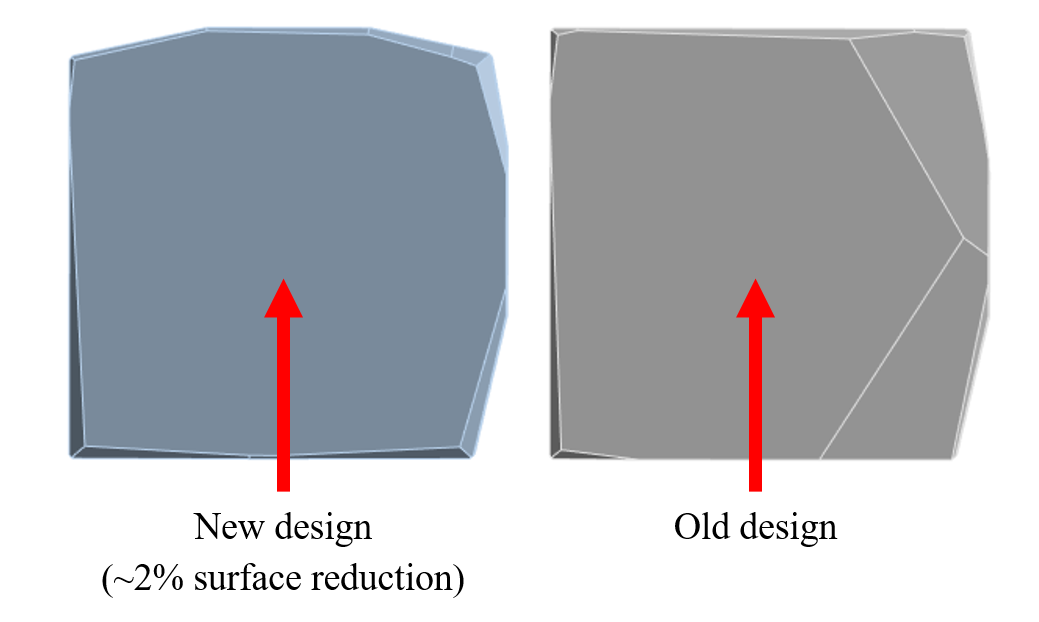
\includegraphics[width=.7\textwidth]{figures/standalonetilemodel.png}
    \caption{\it 3D model of the TZM tiles for integral calculation}
    \label{fig:5.1}
\end{figure}
\\
\break
\normalsize{\indent The idea of this analysis is to apply a heat flux on the plasma facing surface and a set temperature $(20 \si{\degree} C)$ at the back of the tile. This allows to calculate the power needed to assure $(20 \si{\degree} C)$ at the backside of the tile. According to the theory of conductivity, the heat flow entering the tile should be the same as the heat flow evacuated at the back. This can be calculated analytically using the integral form of Fourier's law. ($\it{see}$ \ref{HEAT CONDUCTION THEORY})}
\begin{equation}
    \oiint\displaylimits_{S} \ \mathbf{q} \cdot d \mathbf{S} \ = \ -k\oiint\displaylimits_{S} \ \mathbf{\nabla} T \cdot d \mathbf{S}
    % q_x \ = \ -k \ \partial_x T
    \tagaddtext{[\si{\watt}]}
    \label{eqn:IntFormofFourier}
\end{equation}
\\
\break
\normalsize{\indent The left hand side of the equation \refeq{eqn:IntFormofFourier} is the thermal power $\partial_t Q$ in [$W$] transferred by conduction and defined as $\partial_t Q \ \coloneqq \ \oiint_{S} \ \mathbf{q} \cdot d \mathbf{S}$. The differential $d \mathbf{S}$ is an oriented surface area element in [$m^2$]. On the right hand side of the equation is surface integral of the dot product between the temperature gradient $\mathbf{\nabla} T$ and an oriented surface area element $d \mathbf{S}$. To integrate this equation, it is assumed that the material is homogeneous with constant thermal conductivity. It is then possible to integrate \refeq{eqn:IntFormofFourier} for a 1-D geometry between two points. The result of the integration gives the following expression for heat flow expression:}
\begin{equation}
    %\oiint_{S} \ \mathbf{q} \cdot d \mathbf{S} \ = \ -k\oiint_{S} \ \mathbf{\nabla} T \cdot d \mathbf{S}
    \partial_t Q \ = \ -k \frac{A}{L} \Delta T
    \tagaddtext{[\si{\watt}]}
    \label{eqn:HeatFlow}
\end{equation}
\\
\break
\normalsize{\indent In this expression, $A$ is the cross-sectionnal area perpendicular to the heat flux in [$W$], $L$ is the distance between the two surfaces in [$m$], $\Delta T$ is the temperature difference between both front and back surfaces and $k$ is the thermal conductivity of the medium in [$W/m^2K$]. The cross-sectionnal area $A$ and the length $L$ are assumed constant as well as the thermal conductivity $k$. It is possible to determine the heat flow flowing through the tile and the heat flow evacuated through the boundary condition, they should be equal to satisfy energy conservation. Based on this, it is possible to use a model to approximate the heat flow through the tile.}
\\
\begin{figure}[h!]
    \label{fig_5_2} 
    \centering
    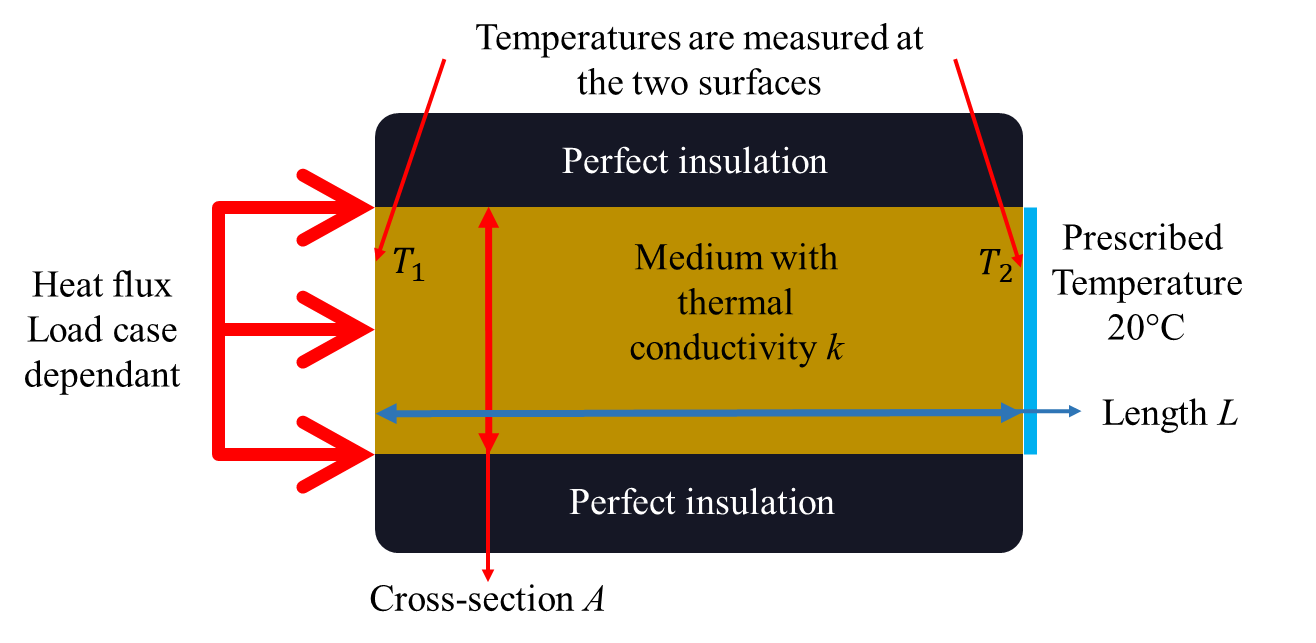
\includegraphics[width=.9\textwidth]{figures/modelforFEcalculationofsurfaceintegral.png}
    \caption{\it Model of the 1-D conduction test}
\end{figure}
\\
\break
\normalsize{\indent According to \refeq{eqn:HeatFlow}, the evolution of the temperature inside the medium is linear. It is then possible to calculate the heat flow flowing in and out (resp. $\partial_t Q_{in}$ and $\partial_t Q_{out}$). The idea is to find what heat flow $\partial_t Q_{out}$ is needed in order to respect the prescribed temperature boundary condition. After some calculations, it was found that $\partial_t Q_{in} \ = \ - \partial_t Q_{out}$. This validates the idea of calculating the surface integral using ANSYS\textsuperscript{\textregistered}. The solver settings of the ANSYS\textsuperscript{\textregistered} project are by default progam controlled. Since the calculation isn't too complex, it is acceptable to continue with these settings. Prescribed temperatures at the back of the \acrshort{TZM} tiles were defined and set to $20 \si{\degree} C$ (it is also important to keep in mind that the backside temperature doesn't affect the value of the integrales, any arbitrary temperature will work).}
\\
\begin{figure}[h!]
    \label{fig_5_3} 
    \centering
    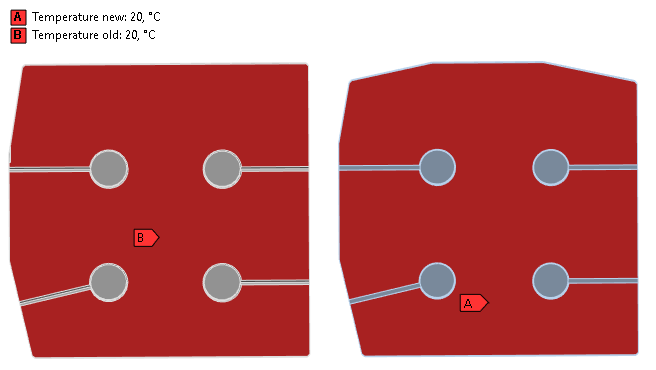
\includegraphics[width=1\textwidth]{figures/surfaceintegraleansysTEMPBC.png}
    \caption{\it Prescribed temperature of the ANSYS\textsuperscript{\textregistered} model for surface integral calculations}
\end{figure}
\\
\break
\normalsize{\indent The loadcases are the standard loadcases chosen to analyse the tile assembly. The were designed to assess the influence of different \acrshort{ECRH} beam heat flux distributions on the thermal behavior of the \acrshort{TZM} tile. They are: }
\\
% INSERT THE SUMMARY TABLE
\begin{table*}[h!]
    \centering
    \ra{1.3}
    %\begin{tabular}{@{}cccc@{}}
    \begin{tabular}{p{4cm}p{1,3cm}p{1,3cm}p{1,3cm}p{2,3cm} }
    \toprule
    $Load \ cases$ & $\makecell{Load \ case \\ number}$ & $\makecell{Plasma \\ radiation}$ & $\makecell{ECRH \\ heat \ load}$ & $\makecell{Film \\ coefficients}$\\
    \cmidrule{1-5}

    %$\makecell{Plasma \ rad. \\ ONLY \\ (Case \ 1) }$ & $yes$ & $no$ & $15 \ \unit{kWm^{-2}\si{\degree}C^{-1}}$\\
    %$\makecell{Plasma \ rad. \ + \\ \acrshort{ECRH} \ axisym. \\ (Case \ 2) }$ & $yes$ & $yes$ & $15 \ \unit{kWm^{-2}\si{\degree}C^{-1}}$\\
    %$\makecell{Plasma \ rad. \ + \\ \acrshort{ECRH} \ non-axisym. \\ (Case \ 3) }$ & $yes$ & $yes^*$ & $15 \ \unit{kWm^{-2}\si{\degree}C^{-1}}$\\
    %$\makecell{Plasma \ rad. \ + \\ \acrshort{ECRH} \ axisym. \\ $[J. Zhu parameters]$ \ $\cite{zhu_parametric_2019}$ \\ (Case \ 4)}$ & $yes$ & $yes^{**}$ & $15 \ \unit{kWm^{-2}\si{\degree}C^{-1}}$\\

    Plasma rad. ONLY & $1$ & $yes$ & $no$ & $15 \ \unit{kWm^{-2}\si{\degree}C^{-1}}$\\
    \myrowcolour%
    Plasma rad.  + \acrshort{ECRH} axisym. & $2$ & $yes$ & $yes$ & $15 \ \unit{kWm^{-2}\si{\degree}C^{-1}}$\\
    Plasma rad. + \acrshort{ECRH} non-axisym. & $3$ & $yes$ & $yes^*$ & $15 \ \unit{kWm^{-2}\si{\degree}C^{-1}}$\\
    \myrowcolour%
    Plasma rad. + \acrshort{ECRH} axisym. [J. Zhu parameters] \cite{zhu_parametric_2019} & $4$ & $yes$ & $yes^{**}$ & $15 \ \unit{kWm^{-2}\si{\degree}C^{-1}}$\\

    % \midrule
\bottomrule
\end{tabular}
\caption{Simulation scenarios, $^{*}$non-axisymmetric heat flux distribution, $^{**}$integration coefficients from J. Zhu \cite{zhu_parametric_2019} }
\label{table:scenarios}
\end{table*}

\normalsize{\indent The integral can be calculated analytically on Wolfram Mathematica\textsuperscript{\textregistered} for the different load cases. The surfaces of the analytical calculations were simplified (to a rectangle) to avoid too complex calculations. It would have been possible to define a Heaviside over a surface defined by an intersection of different linear functions bouding the domain of the surface . The analytical calculations were done to estimate the order of magnitude of the heat flow through the tile. }

\begin{table*}[h!]
    \centering
    \ra{1.3}
    %\begin{tabular}{@{}cccc@{}}
    \begin{tabular}{p{6cm}p{2,4cm}p{2,4cm} }
    \toprule
    $Load \ cases$ & $\makecell{Surface \\ integral \ for \\ old \ design^{*}, \ [ \unit{W}] }$ & $\makecell{Surface \\ integral \ for \\ new \ design^{**}, \ [ \unit{W}] }$ \\
    \cmidrule{1-3}

    Plasma heat load (250 \unit{kWm^{-2} }) & $2700,8$ & $2653,0$\\
    \myrowcolour
    \acrshort{ECRH} axisym. ONLY & $912,0$ & $912,0$\\
    \acrshort{ECRH} non-axisym. ONLY & $791,4$ & $791,4$\\
    \myrowcolour
    Plasma heat load + \acrshort{ECRH} axisym. & $3612,8$ & $3565,0$\\
    Plasma heat load + \acrshort{ECRH} non-axisym. & $3492,2$ & $3444,4$\\

    % \midrule
\bottomrule
\end{tabular}
\caption{Analytical calculations of the surface integrales, $^{*}$Old tile surface = 0,010803 \unit{m^2}, $^{**}$New tile surface = 0,010612 \unit{m^2} }
\end{table*}
\normalsize{\indent The calculation of the surface integrals on ANSYS\textsuperscript{\textregistered} will be compared to the analytical results. They will be used as reference values. The calculations are done with different elemental order (linear and quadratic). In general, for thermal calculations, the elemental order is linear as the results wont change much with respect to the order. }

\begin{table*}[h!]
    \centering
    \ra{1.3}
    % \begin{tabular}{@{}rrrrcrrr@{}}
    \begin{tabular}{p{3,8cm}p{1,5cm}p{1,5cm}p{0,01cm}p{1,5cm}p{1,5cm} }
    \toprule
    Load case & \multicolumn{2}{c}{\makecell{Surface integral for \\ old design, [\unit{W}]} } & \phantom{abc}& \multicolumn{2}{c}{\makecell{Surface integral \\ for new design, [\unit{W}]} }\\
    \cmidrule{2-3} \cmidrule{5-6}
    Element size & $1 \unit{mm}$ & $2 \unit{mm}$ && $1 \unit{mm}$ & $2 \unit{mm}$ \\
    \midrule
    
    %$Linear \ elements$\\
    %\cmidrule{1-1}
    %$1$ & 2700,6 & 2700,6 && 2652,9 & 2652,9\\
    %\myrowcolour
    %$2$ & 3608 & 3607,6 && 3559,4 & 3560,3\\
    %$3$ & 3495,9 & 3495,6 && 3446,8 & 3447,8\\
    %\myrowcolour
    %$4$ & 3612,1 & 3611,5 && 3562,2 & 3562,3\\
    %$Quadratic \ elements$\\
    %\cmidrule{1-1}
    %$1$ & 2700,6 & 2700,6 && 2652,9 & 2652,9\\
    %\myrowcolour
    %$2$ & 3607,2 & 3607,4 && 3559,4 & 3560,5\\
    %$3$ & 3495,6 & 3495,7 && 3446,9 & 3447,6\\
    %\myrowcolour
    %$4$ & 3611,8 & 3611,3 && 3562,2 & 3562,4\\

    $Linear \ elements$\\
    \cmidrule{1-1}
    Plasma heat load ONLY & 2700,6 & 2700,6 && 2652,9 & 2652,9\\
    \myrowcolour
    Plasma rad.  + \acrshort{ECRH} axisym. & 3608,0 & 3607,6 && 3559,4 & 3560,3\\
    Plasma rad. + \acrshort{ECRH} non-axisym. & 3495,9 & 3495,6 && 3446,8 & 3447,8\\
    \myrowcolour
    Plasma rad. + \acrshort{ECRH} axisym. [J. Zhu parameters] \cite{zhu_parametric_2019} & 3612,1 & 3611,5 && 3562,2 & 3562,3\\
    
    $Quadratic \ elements$\\
    \cmidrule{1-1}
    Plasma heat load ONLY & 2700,6 & 2700,6 && 2652,9 & 2652,9\\
    \myrowcolour
    Plasma rad.  + \acrshort{ECRH} axisym. & 3607,2 & 3607,4 && 3559,4 & 3560,5\\
    Plasma rad. + \acrshort{ECRH} non-axisym. & 3495,6 & 3495,7 && 3446,9 & 3447,6\\
    \myrowcolour
    Plasma rad. + \acrshort{ECRH} axisym. [J. Zhu parameters] \cite{zhu_parametric_2019} & 3611,8 & 3611,3 && 3562,2 & 3562,4\\

    \bottomrule
\end{tabular}
\caption{Finite element calculations of the surface integrales using the model \ref{fig:5.1}}
\end{table*}

\normalsize{\indent There are a few things that can be discussed. Firstly the elemental order doesn't drastically change value of the integral (the value of the integral changes by about 0,1 \unit{W} between linear and quadratic elements). For the thermal analysis of the whole tile assembly, linear elements will be used to mesh the geometries. Another parameter is the element size that varies between 1 and 2 \unit{mm} and the variation also doesn't affect the results (the surface integrales vary by about $max.$ 1 \unit{W}). The numerical calculations allow to verify the analytical calculations and show little variation between values with only about 0,08 \% variation of heat flow in average between the two calculations methods.}
\\
\break
\normalsize{\indent The surface integrales of the two design can also be used to assess the decrease of heat flow through the surfaces.}

\subsection{Comparison between old and new TZM tile design}
\normalsize{The surface integrales of the two design can also be used to assess the decrease of heat flow through the surfaces. It is also possible to calculate the energy balance to check the validity of the calculation. Analytically, it is already possible to see the decrease in power flow through the tile. This approximately 1,7 \% decrease in power flow is in accordance to the 2 \% surface area decrease. The geometry change does have the desired effect.}
\\
\begin{figure}[h!]
    \label{fig_5_6} 
    \centering
    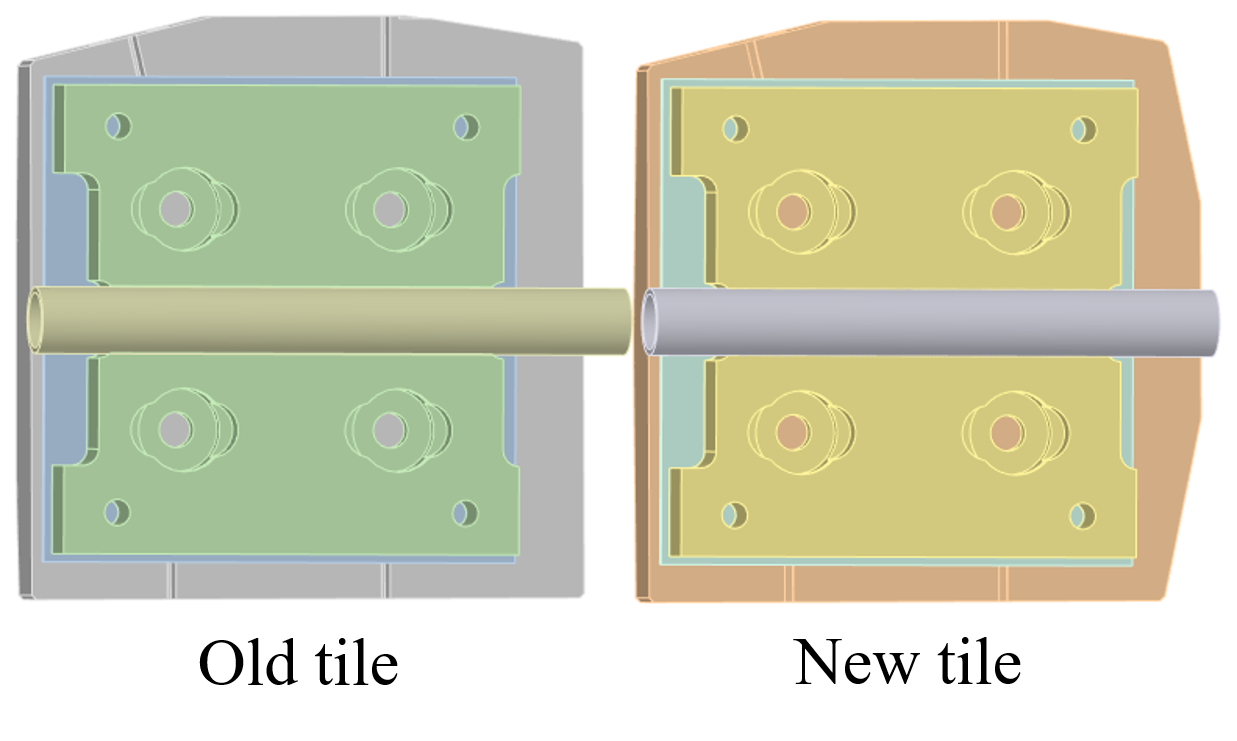
\includegraphics[width=.51\textwidth]{figures/energybalancemodel.png}
    \caption{\it Prescribed temperature of the ANSYS\textsuperscript{\textregistered} model for surface integral calculations}
\end{figure}
\\
\normalsize{\indent The four load cases ({\it see table \ref{table:scenarios}}) were calculated for the tile assembly. The radiation on the plasma-side and \acrshort{PV}-side of the \acrshort{TZM} tile as well as the \acrshort{CuCrZr} heat sink and \acrshort{SS} cooling pipe is applied.}
\\
\break
\normalsize{\indent The calculations are done and the reaction of the boundary conditions is calculated and summed ($\Sigma Power_{out}$) and compared to the \acrshort{FE} calculations. So it is possible to validate the numerical model:}

\begin{table*}[h!]
    \centering
    %\caption{Power conservation summary table}
    \label{table:5.4}
    \ra{1.3}
    %\begin{tabular}{@{}cccc@{}}
    \begin{tabular}{p{6cm}p{2cm}p{2cm} }
    \toprule
    $Load \ cases$ & $\makecell{Surface \\ integral, \ [ \unit{W}] }$ & $\makecell{\Sigma Power_{out}, \ [ \unit{W}] }$ \\
    \cmidrule{1-3}

    Plasma heat load (250 \unit{kWm^{-2} }) & $2652,9$ & $2652,9$\\
    \myrowcolour
    Plasma heat load + \acrshort{ECRH} axisym. & $3560,3$ & $3559,8$\\
    Plasma heat load + \acrshort{ECRH} non-axisym. & $3447,8$ & $3450,4$\\
    \myrowcolour
    Plasma rad. + \acrshort{ECRH} axisym. [J. Zhu parameters] \cite{zhu_parametric_2019} & $3562,3$ & $3562,2$\\

    % \midrule
\bottomrule
\end{tabular}
\caption{Power conservation summary table}
\end{table*}

\normalsize{\indent The calculation of the whole tile assembly provided good insight on the temperature distribution within the \acrshort{TZM} tile and the \acrshort{CuCrZr} heat sink. It is possible to see the temperature reduction as an effect of a lower exposed surface area of the \acrshort{TZM} tile. The temperature of the heat sink is also lower for the new design than the older one. The design change of the \acrshort{TZM} reflector tile thus have an effect on the temperature fields of the assembly parts. {\bfseries It is also important to keep in mind that the convection coefficient is set to 30 \unit{kWm^{-2}\si{\degree}C^{-1}}, which is not realistic}. This was assumed to compare the old calculations with the new model.}
\\
\begin{figure}[h!]
    \label{fig_5_4} 
    \centering
    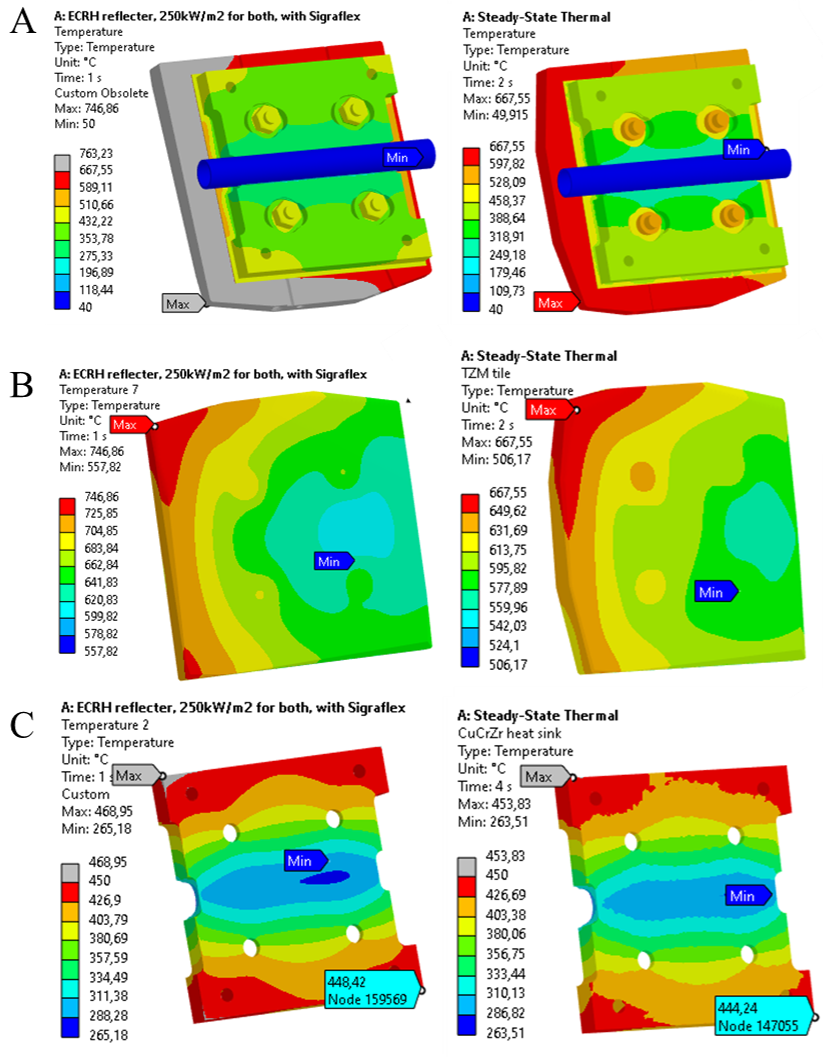
\includegraphics[width=.9\textwidth]{figures/OLDVSNEWTEMPERATUREFRINGES.png}
    \caption{\it Temperature fields for resp. old and new design. Viwa A is the entire model, view B is just the \acrshort{TZM} reflector tile and view C is the \acrshort{CuCrZr} heat sink.}
\end{figure}
\\
\normalsize{\indent The power conservation is indeed respected and it is possible to conclude several points:
    \begin{itemize}
        \item The power conservation is respected and validates the numerical model.
        \item The analytical and numerical calculations show that the new design (reduction of the \acrshort{TZM} tile surface area) reduced power flow through the assembly by about 1,85 \% the initial power of the plasma heat load (\acrshort{ECRH} heat flux being small near the edges of the \acrshort{TZM} tile, it doesnt affect much the integral heat flow).
        \item The new design also lowered the temperature of all assembly parts, especially the \acrshort{CuCrZr} heat sink with a decrease of about 3,33 \% of initial design temperature.
    \end{itemize}
}

\subsection{Film coefficient influence on thermal behavior}
\normalsize{After calculating the surface integrales, it is possible to perform the thermal analysis for the different film ceofficients to assess the influence of it on the temperature field inside of the assembly parts. The calculations were perfomed used the model defined in chapter \ref{chapter:3.1}. Early calculations without \acrshort{ECRH} heat load showed non-negligible influence of film coefficient variations on thermal behavior of the \acrshort{TZM} reflector tile assembly. The film coefficient's value was swept and only the lowest and highest were graphed as they are the most interesting points.}
\\
\begin{figure}[h!]
    \label{fig_5_7} 
    \centering
    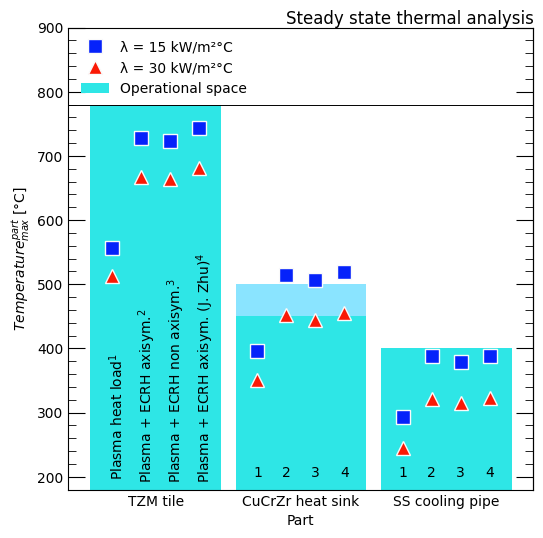
\includegraphics[width=.6\textwidth]{figures/filmcoefficient15and30.png}
    \caption{\it Maximum part temperature in function of load case. The maximum operational temperature is not fixed for \acrshort{CuCrZr}.}
\end{figure}
\\
\normalsize{\indent It is possible to assess the temperature differences on the temperature fringe of the ANSYS\textsuperscript{\textregistered} Mechanical post-processor. The lowest film coefficient (the one most likely to be attained during operation) is not enough to keep the heat sink from overheating (if said maximum operational temperature of \acrshort{CuCrZr} is set to 450 \unit{\si{\degree}C}).Another temperature limit discussed with Axel Lorenz was set to 500 \unit{\si{\degree}C} (after the \acrshort{CuCrZr} was tested at the Karlsruhe Institute for Technology and no signs of considerable damage was seen).}
\begin{figure}[h!]
    \label{fig_5_8} 
    \centering
    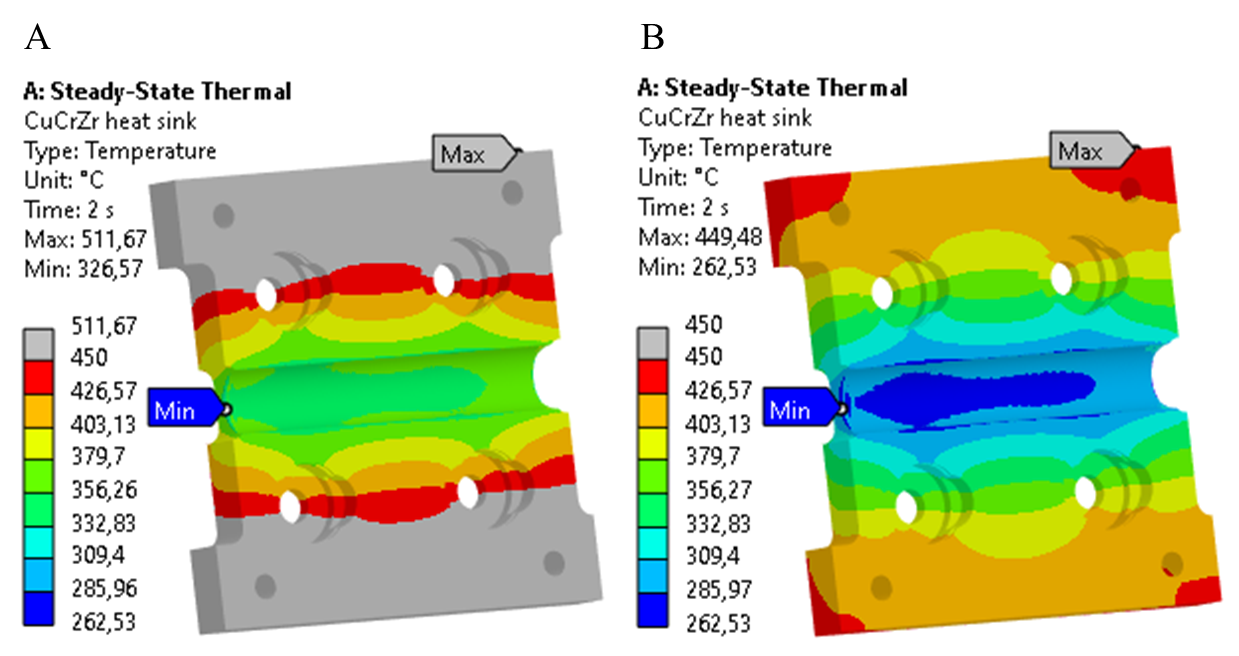
\includegraphics[width=.7\textwidth]{figures/filmcoefficient15and30TEMPERATREFRINGEHS.png}
    \caption{\it Maximum heat sink temperature for two film coefficients. View A is the old \acrshort{TZM} reflector tile design's heat sink and view B is the new \acrshort{TZM} reflector tile design's heat sink}
\end{figure}
\\
\normalsize{\indent The maximum temperature of the heat sink at 15 \unit{kWm^{-2}\si{\degree}C} exceeds the maximum temperature of 450 \unit{\si{\degree}}C \cite{Fellinger_2013} \cite{zhu_parametric_2019} by about 13,7 \% (511,67 \unit{\si{\degree}}C). If the maximum temperature was set to be 500 \unit{\si{\degree}}C, the lowest film coefficient still wouldn't allow 250 \unit{kWm^{-2}}. {\bfseries It is possible to conclude that the film coefficient range stated by J. Fellinger is not enough to keep the heat sink from overheating/recrystallizing.}}
\subsection{Load case influence on thermal behavior} \label{Load case influence on thermal behavior}
% \Huge{AAAAAAAAAAAAAAAAAAAAAAAAAAAAAAAAAAAAAAAAAAAAAAAAHHHHHHHHHHHHHHHHH}
\normalsize{To gain more insight on the thermal behavior of the tile assembly and characterize its functionning, it is possible to perform static thermal analysis for various load cases, namely the load cases explained in table \ref{table:5.4}. The film coefficient used fore these calculations is the low 15 \unit{kWm^{-2}\si{\degree}C}. }
\\
\begin{figure}[h!]
    \label{fig_5_10} 
    \centering
    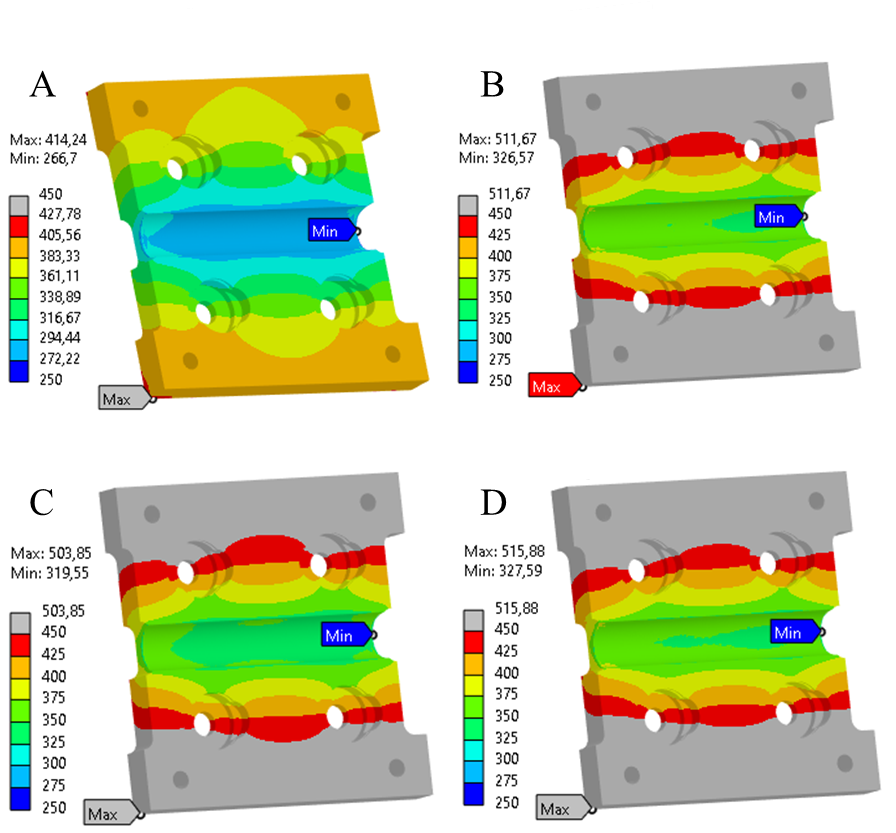
\includegraphics[width=.7\textwidth]{figures/loadcasestaticthermalHSTF.png}
    \caption{\it Maximum heat sink temperature in function of load case. View A is for plasma heat load ONLY case, View B is for plasma heat load + ECRH axisymmetric heat load, View C is for plasma heat load + ECRH NON-axisymmetric heat load  and View C is for plasma heat load + ECRH axisymmetric heat load with J. Zhu parameters.}
\end{figure}
\\
\normalsize{\indent For the first case, there is no overheating of the heat sink. For the three other cases, the heat sink overheats with the last case (the ECRH heat load with the parameters from J. Zhu) being the worst with the highest maximum temperature. In all cases with ECRH beam on, a big fraction of the heat sink exceeds the maximum operational temperature. The issue of the recrystallization of the bronze alloy was discussed and deemed NOT necessarily problematic since the temperature of 450 \unit{\si{\degree}C} can be exceeded and it was stated during a discussion with Axel Lorenz that the alloy can be used beyond this temperature. While it is possible to simulate accurate metallurgical phase changes, it is nontheless complicated to model due to lack of metallurgical and thermodynamical properties.}
\\
\break
\normalsize{\indent Because this analysis a a static analysis, the temperature field satisfies the thermal equilibrium equation $0=-\alpha \nabla T$. It is possible to perform a transient thermal analysis to determine the critical time at which temperature is exceeded for the ONE of the parts and check the evolution of the temperature field for different pulse durations.}